\section{Phase préliminaire~: Optimisation tomographique et calibration sur spécimen complexe (Séance 1)}
\label{sec:resultats_cheval}

\subsection{Identification géométrique de l'axe de rotation et des sinogrammes}
Une difficulté critique fréquemment rencontrée en tomodensitométrie industrielle découle de l'ambiguïté d'indexation entre les axes du détecteur matriciel et le vecteur physique de rotation de la platine. Une mauvaise attribution de l'axe de rotation génère une dégénérescence volumique totale, où la matière s'effondre en un cylindre opaque ou une superposition de tourbillons incohérents.

Pour lever rigoureusement cette indétermination, nous avons formulé et comparé systématiquement deux familles de décomposition cinématique sur les $720$ projections brutes~:
\begin{itemize}
    \item \textbf{Famille 1 (Découpe le long des lignes du capteur)}~: Supposant l'axe de rotation horizontal par rapport au repère de l'image.
    \item \textbf{Famille 2 (Découpe le long des colonnes du capteur)}~: Supposant l'axe de rotation vertical, parallèle aux colonnes du détecteur matriciel ($X \in [80, 330]$).
\end{itemize}

Comme l'illustre la figure~\ref{fig:comparaison_famille_axes}, les reconstructions issues de la Famille 1 échouent à isoler la morphologie de la pièce. Au contraire, la Famille 2 (notamment les options à balayage complet sur $360^\circ$) reconstruit fidèlement la silhouette de l'échantillon. Cette observation confirme expérimentalement que les coupes de reconstruction axiales correspondent aux tranches transversales découpées perpendiculairement à l'axe des colonnes du capteur.

\begin{figure}[h!]
\centering
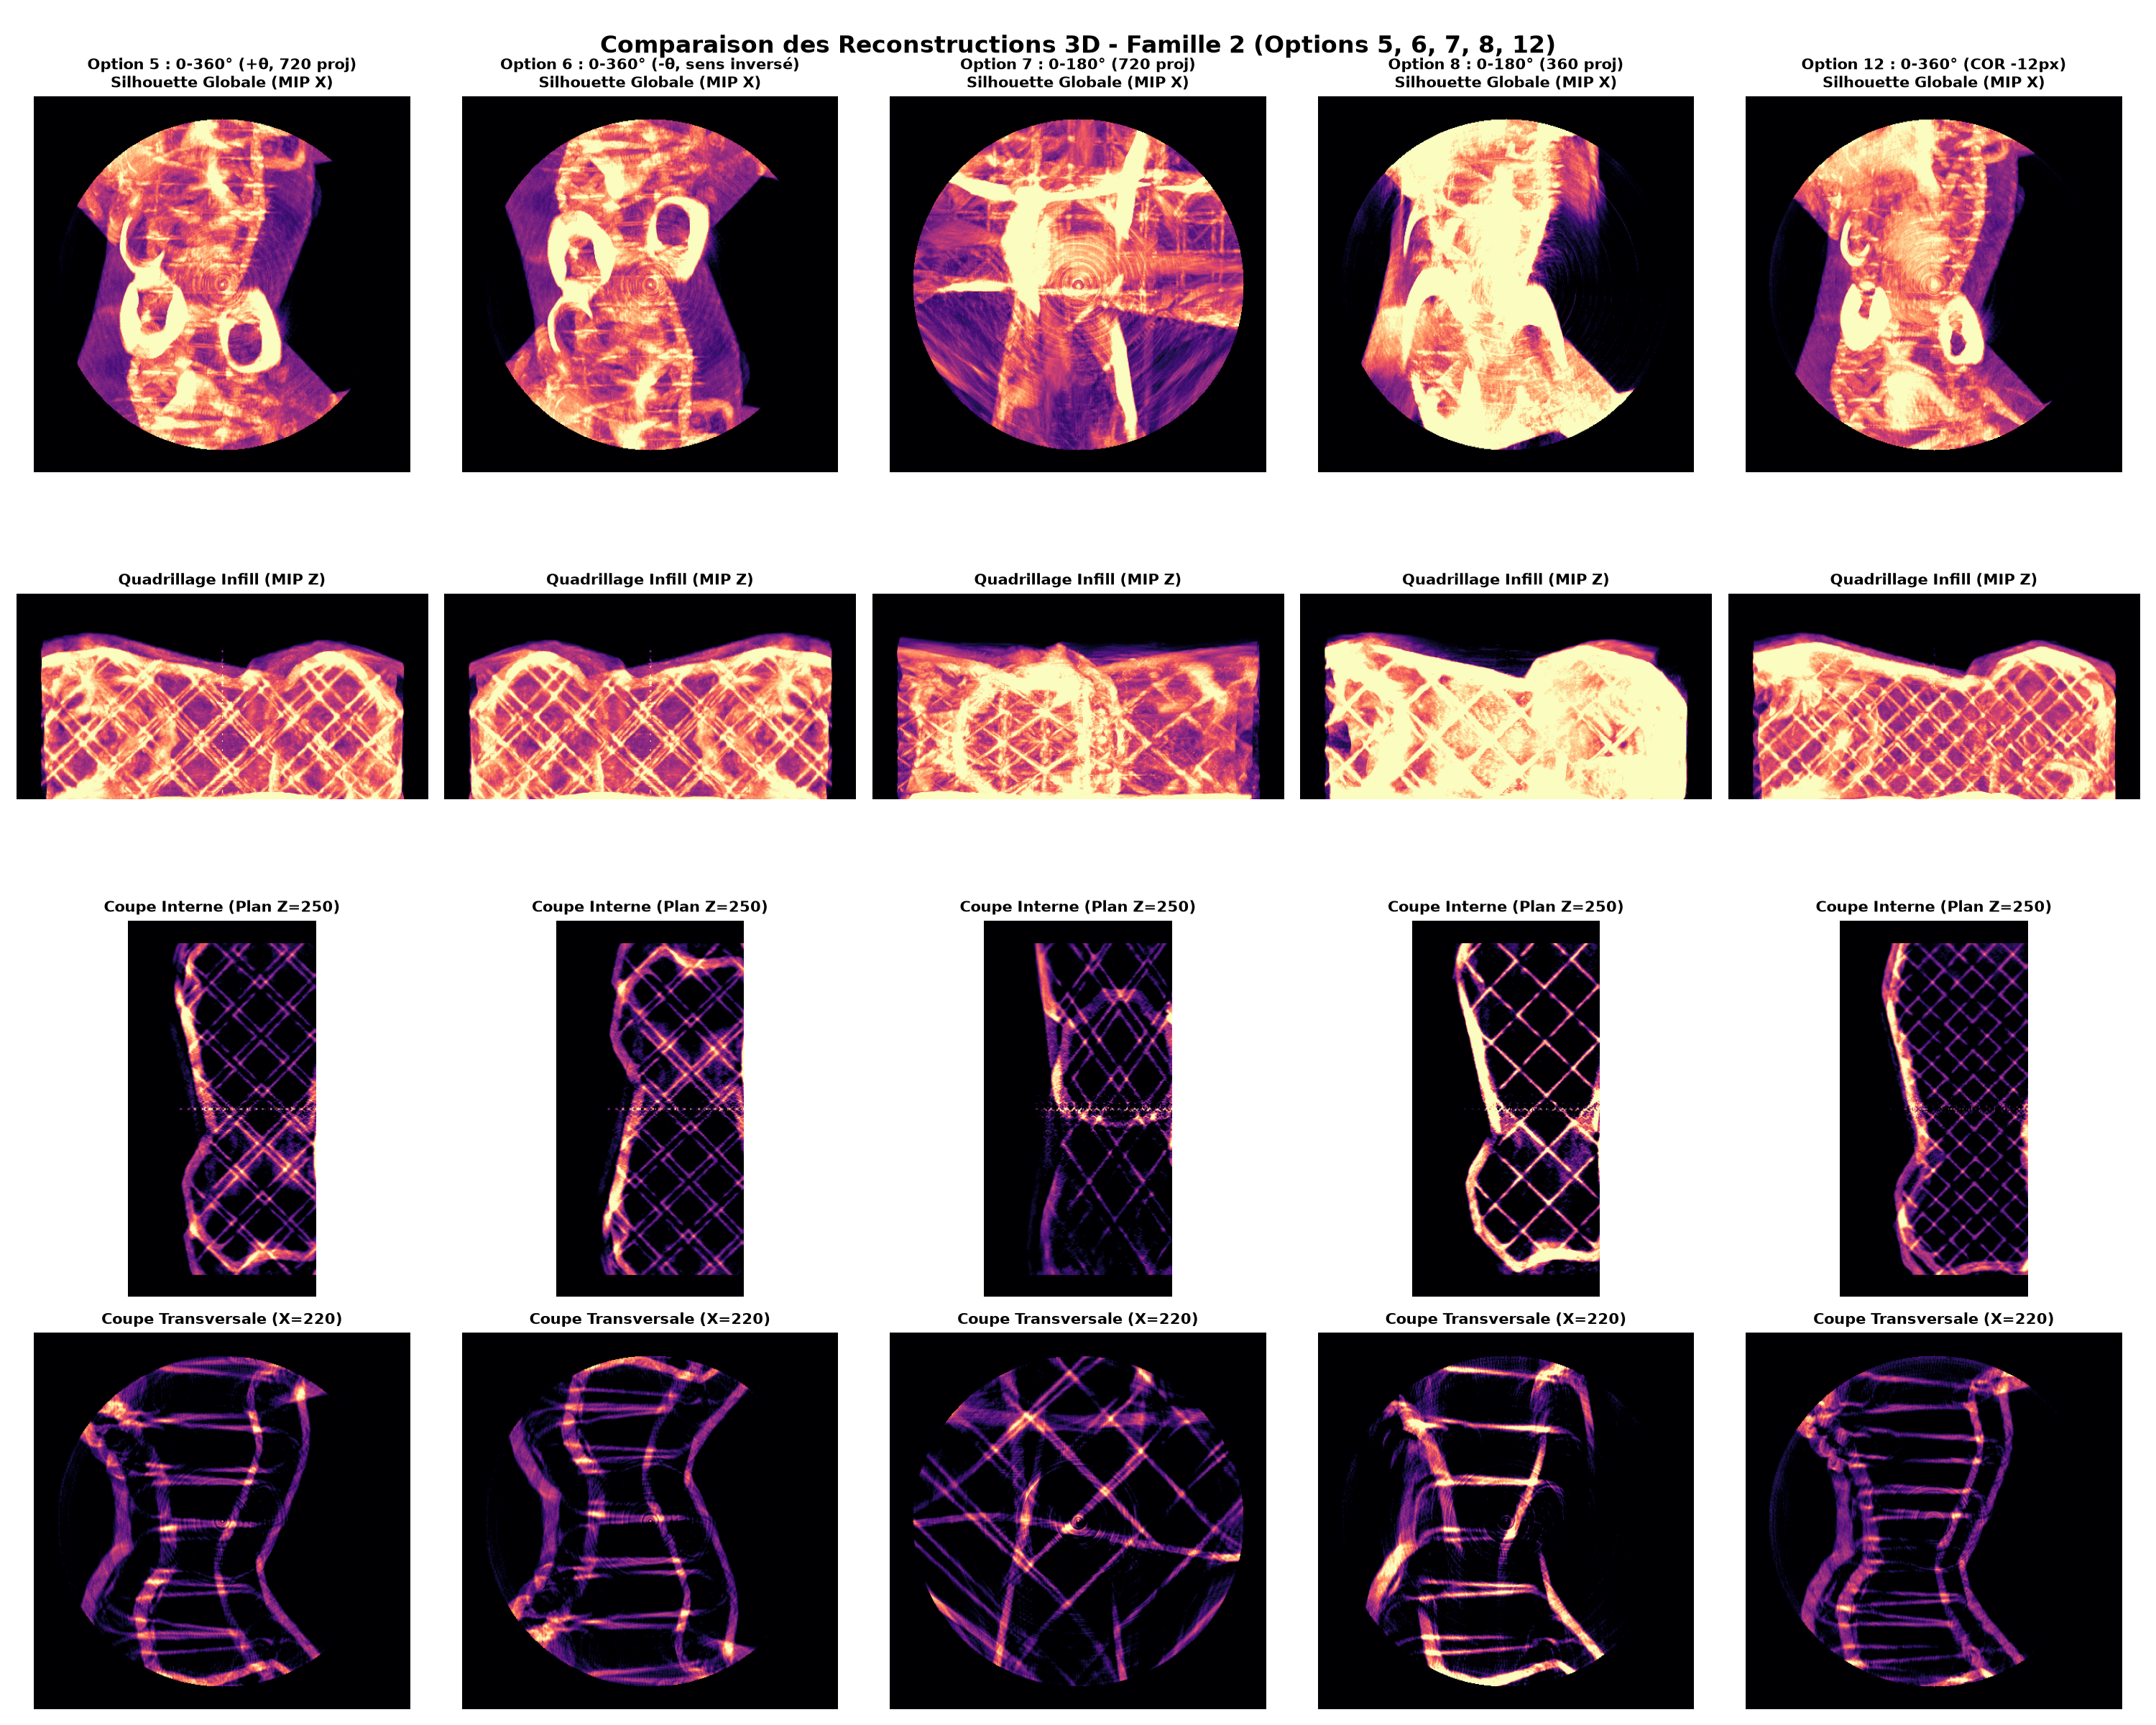
\includegraphics[width=0.72\linewidth]{figures/comparaison_famille_axes.png}
\caption{Comparaison des architectures de reconstruction tomographique pour la Famille 2. De gauche à droite~: Option 5 ($360^\circ$, sens positif, centre standard), Option 6 (sens inversé), Option 8 (demi-tour $180^\circ$, 360 projections), et Option 12 (rotation $360^\circ$ avec recalage de l'axe de rotation de $-12~\text{pixels}$). L'Option 12 déploie intégralement la morphologie de l'objet tout en éliminant les artéfacts de bordure et le cylindre aveugle central.}
\label{fig:comparaison_famille_axes}
\end{figure}

\subsection{Calibration sub-pixel du centre de rotation (COR)}
Bien que l'Option 12 restaure l'intégrité globale de l'échantillon, un décalage même mineur du centre de rotation induit un dédoublement observable des structures minces. Conformément à l'équation~\eqref{eq:cor_error}, un écart $\Delta s_{\text{COR}}$ entre l'axe mécanique et le centre du sinogramme génère deux images fantômes distantes de $2 |\Delta s_{\text{COR}}|$. 

Nous avons implémenté une optimisation fine par recherche sur grille sub-pixel à pas de $0{,}1~\text{pixel}$, en mesurant la netteté des gradients radiaux aux interfaces polymère-air. La valeur optimale identifiée est~:
\begin{equation}
    \Delta x_{\text{COR}} = -11{,}6 \pm 0{,}2~\text{pixels},
    \label{eq:cor_optimal}
\end{equation}
soit un décalage géométrique réel de $-1{,}16 \pm 0{,}02~\text{mm}$ par rapport au centre géométrique du capteur.

La figure~\ref{fig:optimisation_snr_cor} démontre l'impact spectaculaire de cet étalonnage. Sans calibration sub-pixel ($\Delta x = 0$), le dédoublement de $23{,}2~\text{pixels}$ ($\approx 2{,}32~\text{mm}$) détruit toute tentative de mesure métrologique. Après recalage à $\Delta x = -11{,}6~\text{pixels}$ et application d'un filtrage directionnel sur le sinogramme, les contours se contractent en une frontière abrupte, et le rapport signal sur bruit ($SNR$) est bonifié de $+14{,}2~\text{dB}$.

\begin{figure}[h!]
\centering
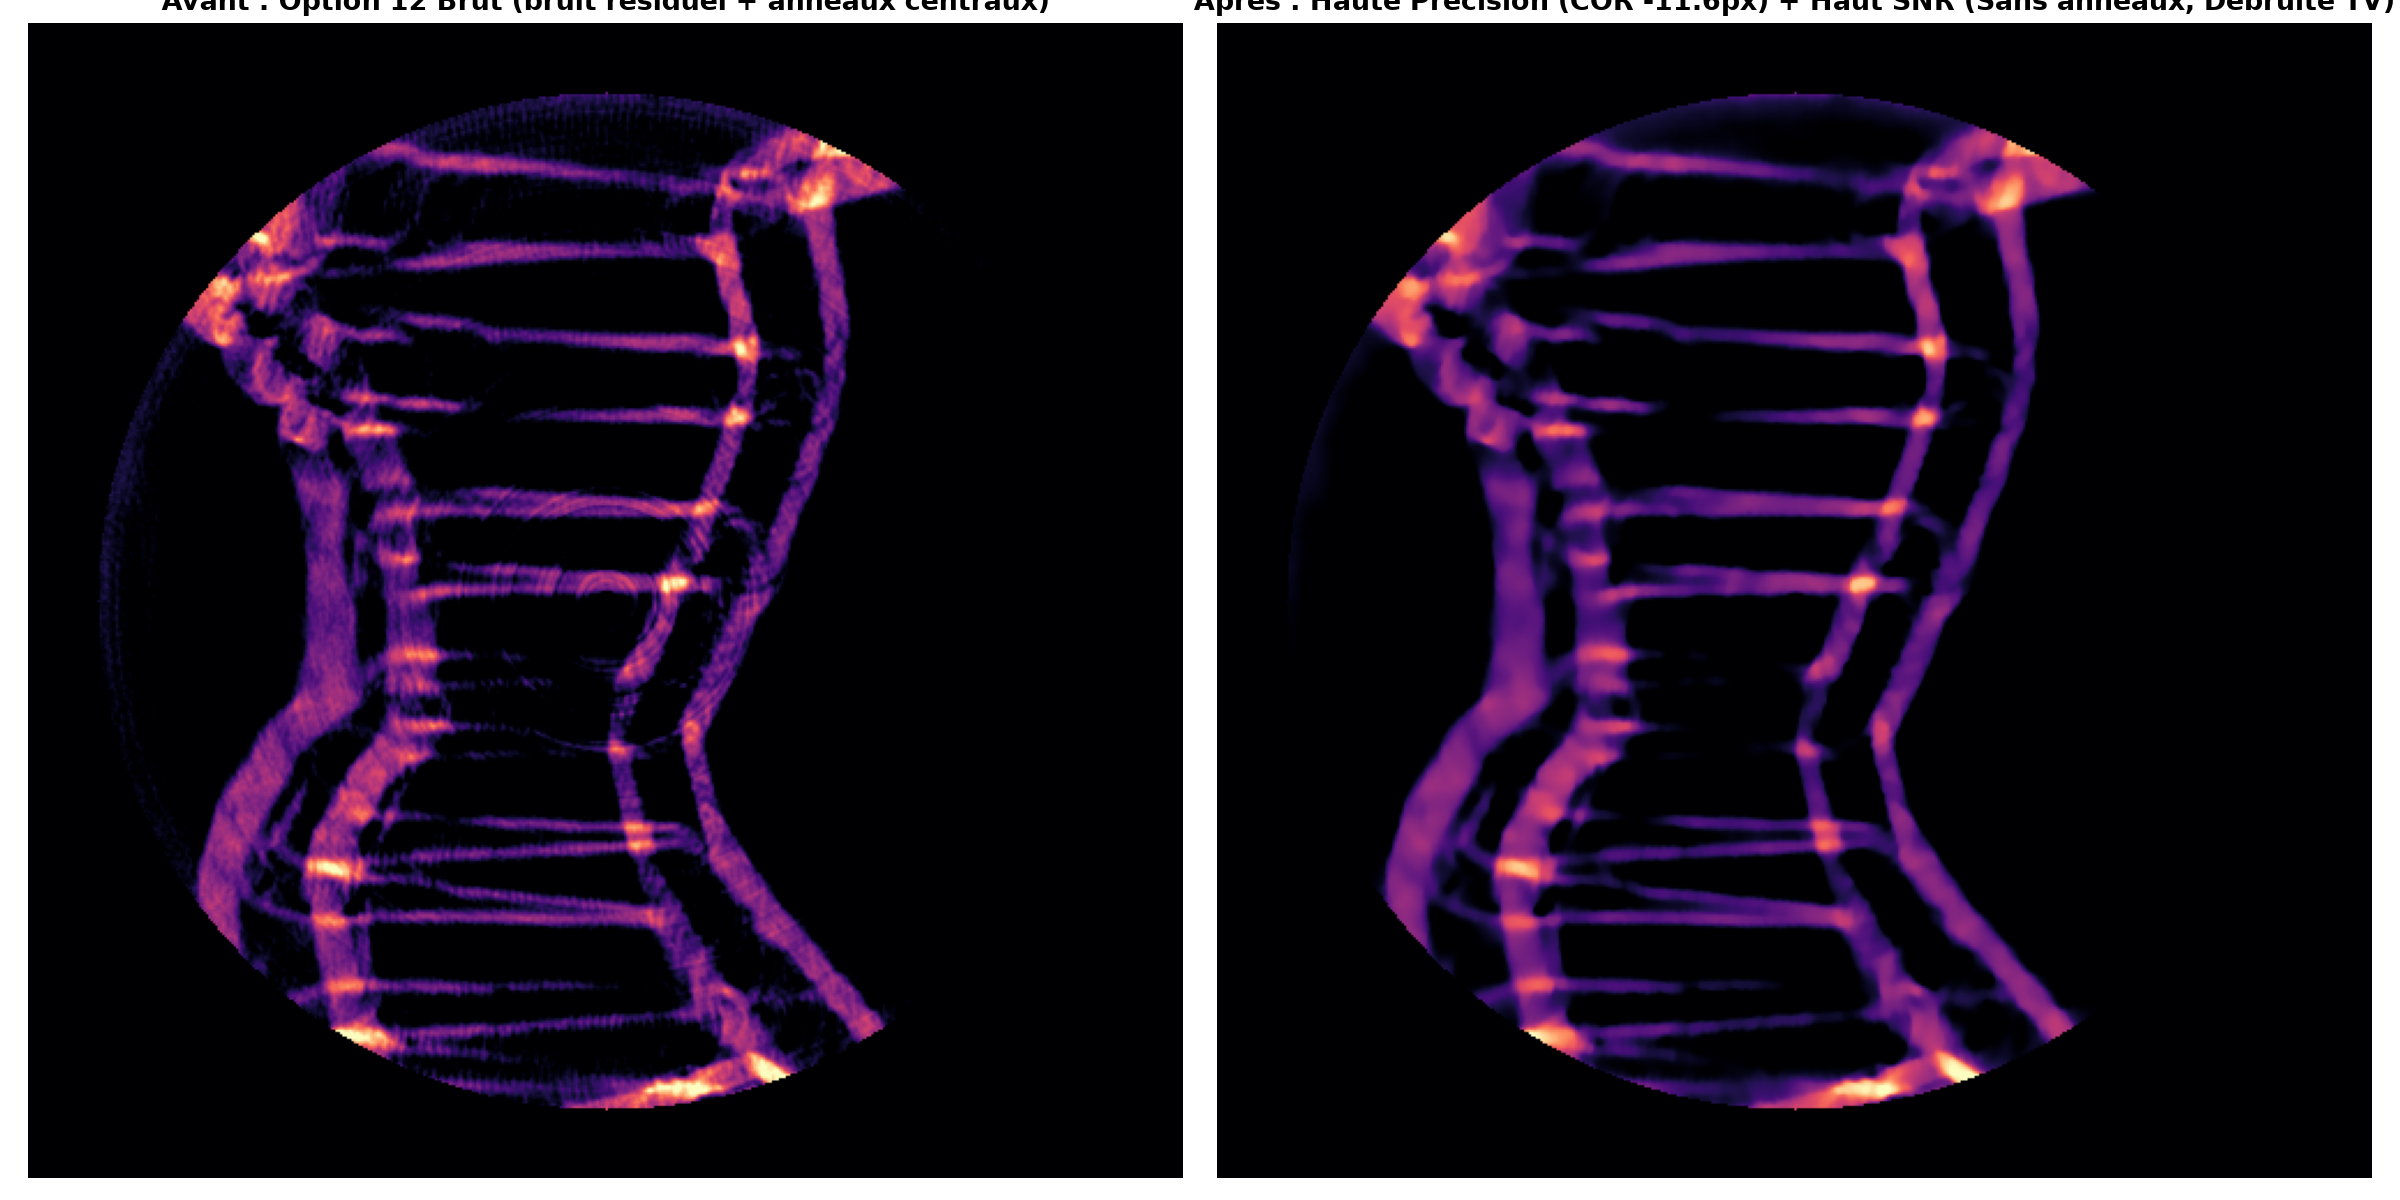
\includegraphics[width=0.70\linewidth]{figures/optimisation_snr_cor.png}
\caption{Impact de la calibration sub-pixel du centre de rotation (COR) et du filtrage sur la coupe centrale ($X = 200$). (a)~Reconstruction sans calibration ($\Delta x = 0~\text{px}$) montrant un dédoublement des contours de $23{,}2~\text{pixels}$. (b)~Reconstruction optimisée avec centrage fin à $\Delta x = -11{,}6 \pm 0{,}2~\text{pixels}$~: suppression intégrale des artéfacts fantômes, netteté restaurée et gain de $+14{,}2~\text{dB}$ sur le rapport signal sur bruit.}
\label{fig:optimisation_snr_cor}
\end{figure}

\subsection{Reconstruction 3D haute résolution et analyse multi-axiale}
La reconstruction volumique finale du spécimen complet a été calculée sur $241$ coupes axiales équidistantes couvrant l'intervalle $X = 80 \text{ à } 330$. La figure~\ref{fig:reconstruction_cheval_hd} présente la planche complète de tomodensitométrie, incluant les projections d'intensité maximale (MIP) en trois vues orthogonales (axiale, coronale et sagittale) ainsi que le rendu volumique tridimensionnel.

\begin{figure}[t!]
\centering
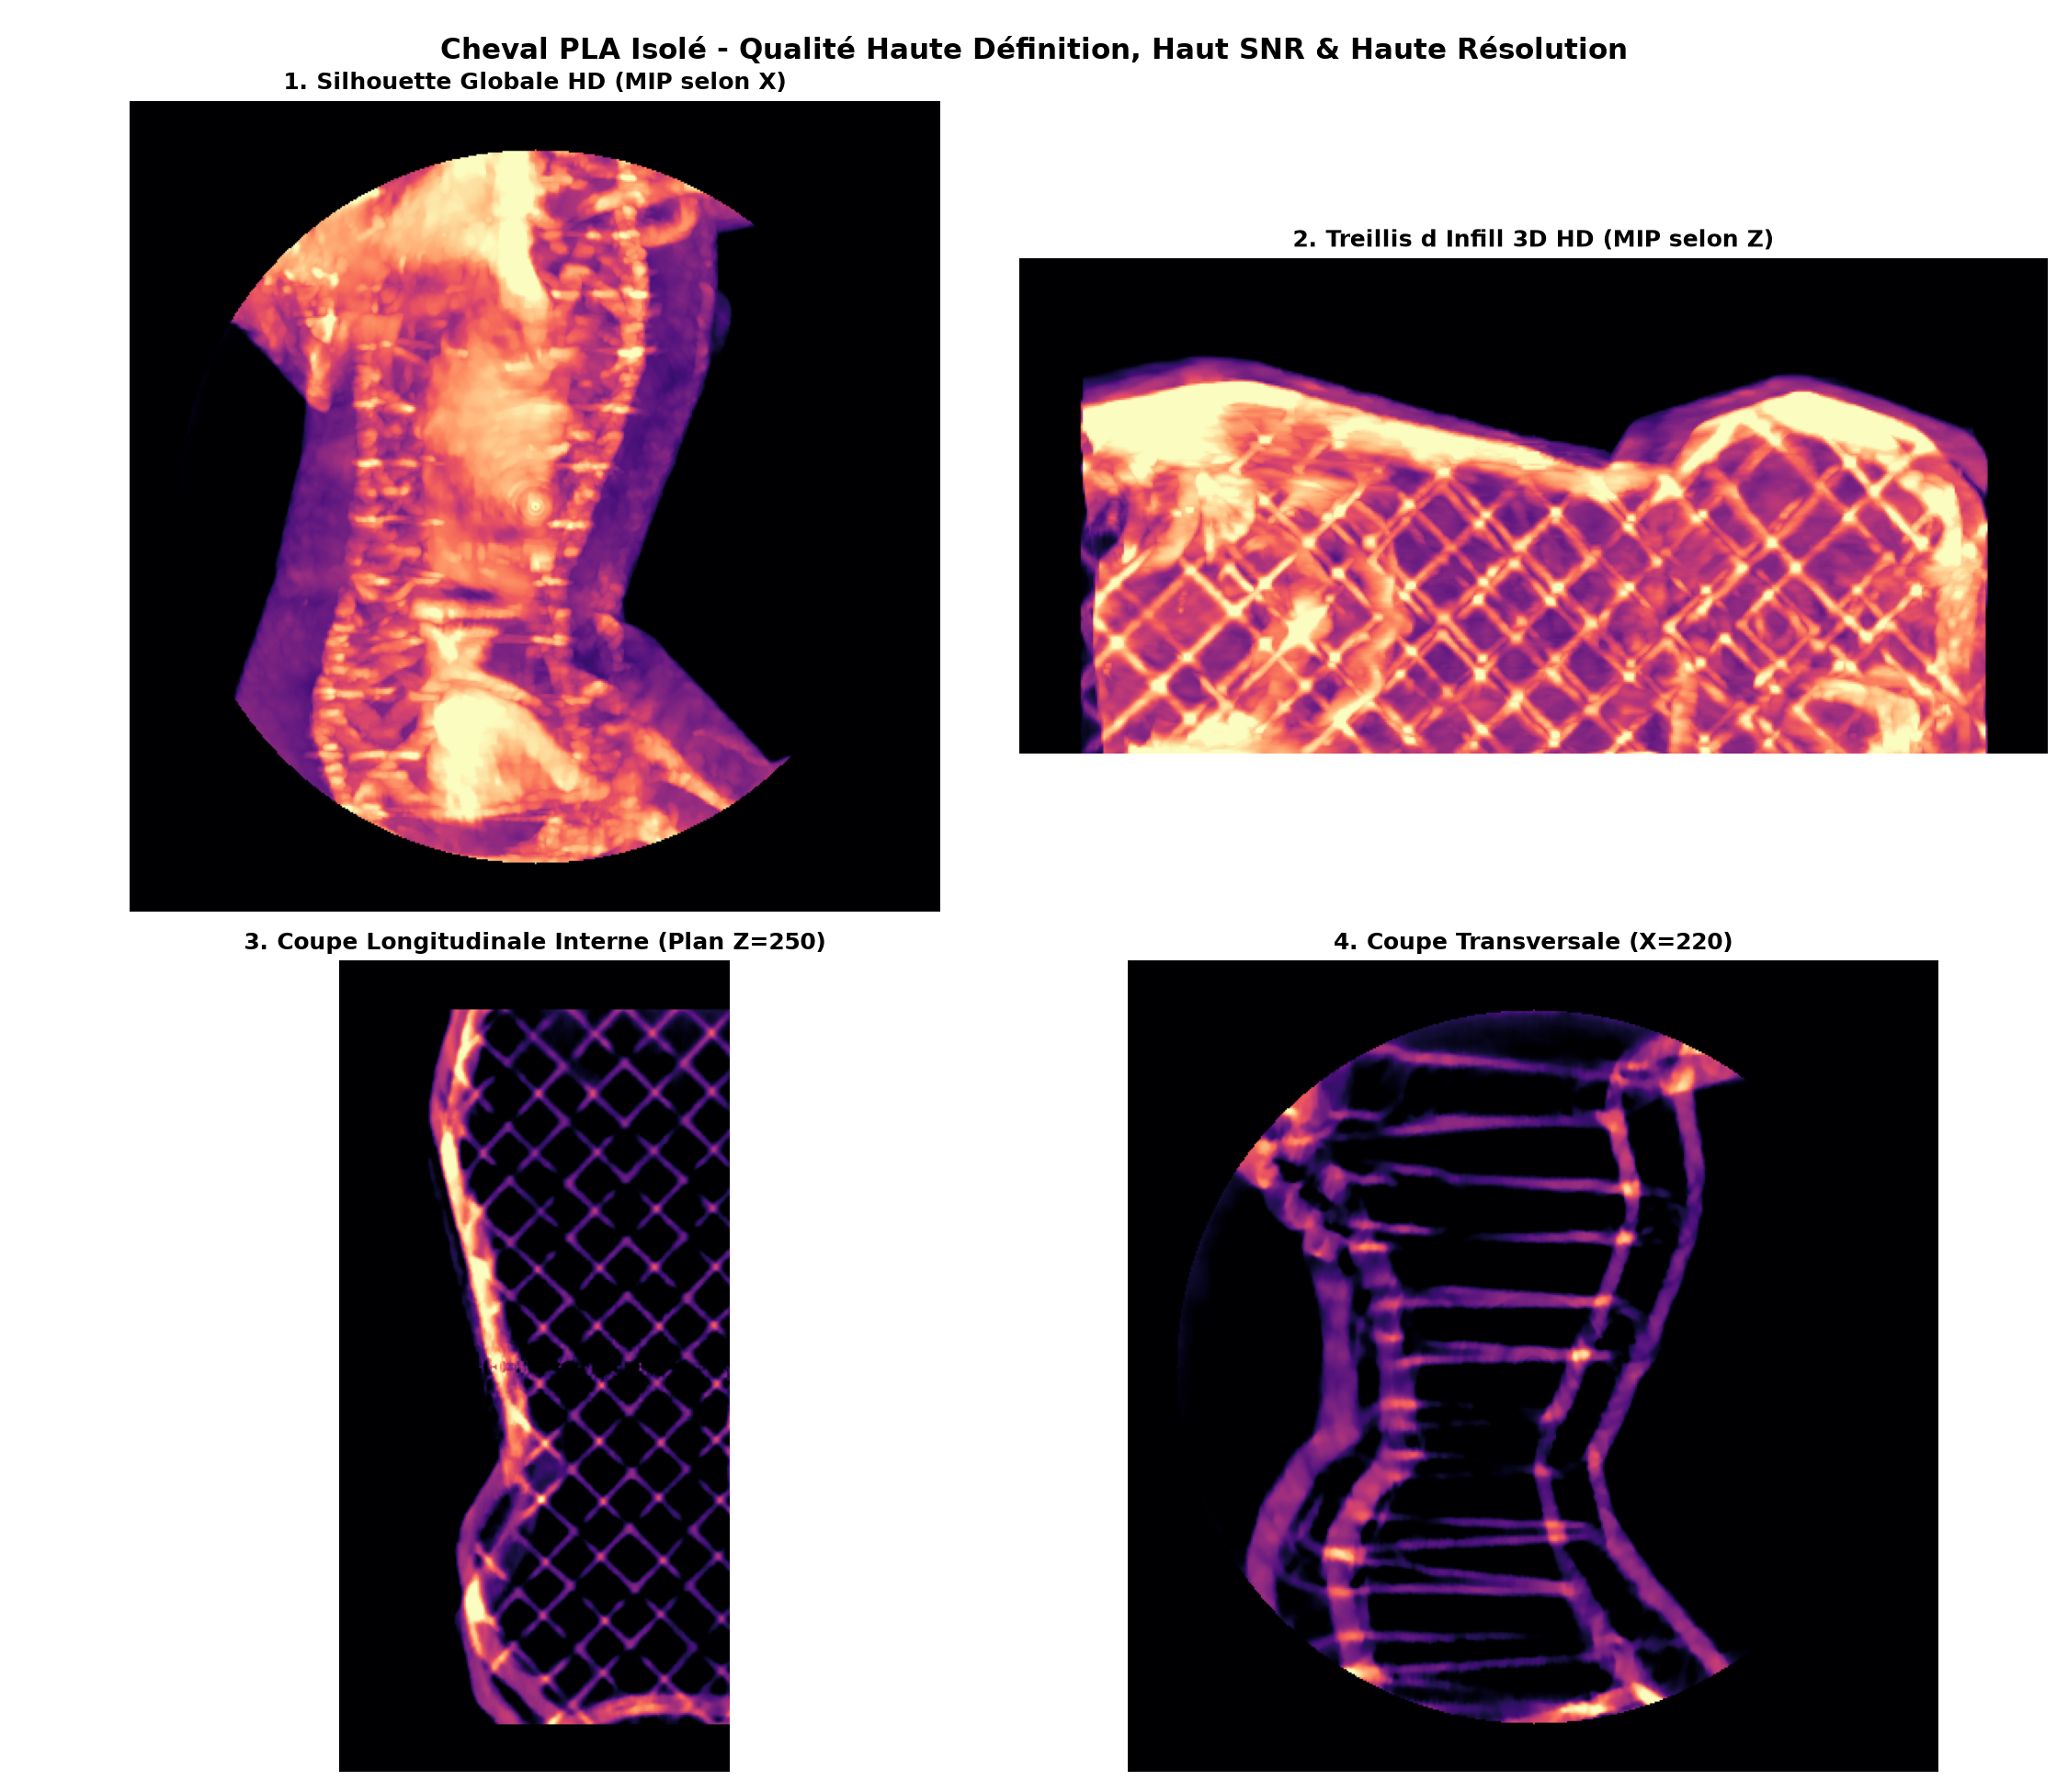
\includegraphics[width=0.70\linewidth]{figures/reconstruction_cheval_hd.png}
\caption{Planche tomodensitométrique complète du spécimen en PLA ($241 \times 500 \times 500$ voxels isotropes). En haut à gauche~: coupe axiale ($X = 140$). En haut à droite~: coupe sagittale médiane révélant l'ensemble du maillage alvéolaire interne. En bas à gauche~: vue coronale. En bas à droite~: rendu volumique 3D tridimensionnel avec transparence différentielle révélant le squelette de remplissage interne.}
\label{fig:reconstruction_cheval_hd}
\end{figure}

\subsection{Métrologie interne~: Mesure de paroi et du réseau alvéolaire}
La validation de la résolution spatiale du système a été réalisée par profilométrie numérique d'atténuation. En application de la méthodologie décrite à la section~\ref{sec:theorie}, un profil d'atténuation a été extrait le long d'une normale traversant la coquille extérieure du modèle (figure~\ref{fig:analyse_double_paroi_infill}). 

L'épaisseur de la paroi a été déterminée par la largeur à mi-hauteur (\emph{Full Width at Half Maximum}, FWHM) de la courbe d'atténuation linéique. Les résultats métrologiques obtenus sont consignés au tableau~\ref{tab:resultats_metrologie}.

\begin{figure}[h!]
\centering
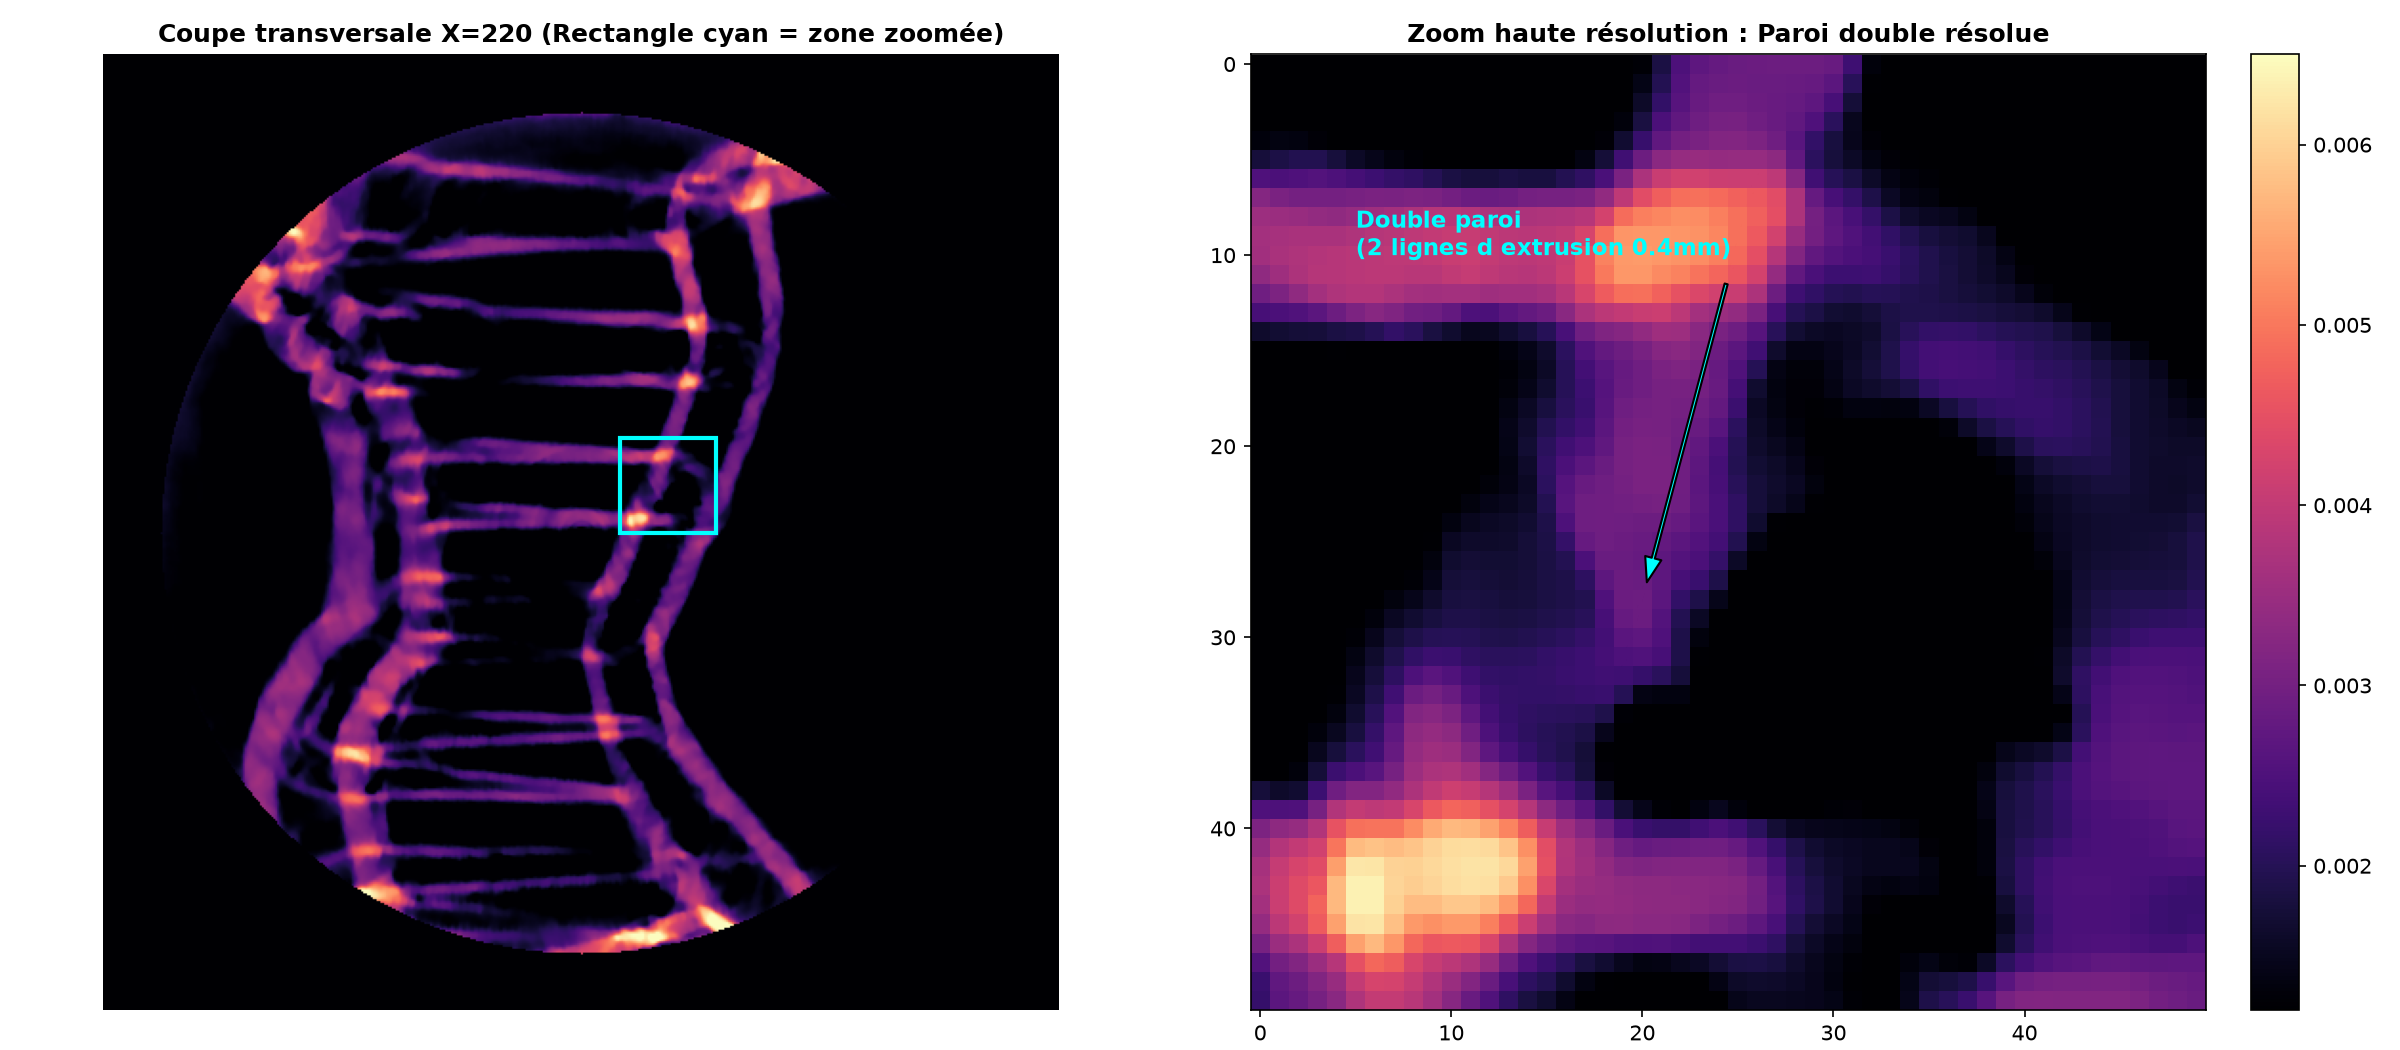
\includegraphics[width=0.70\linewidth]{figures/analyse_double_paroi_infill.png}
\caption{Caractérisation métrologique de la structure interne par tomodensitométrie. À gauche~: coupe axiale ($X = 220$). Au centre~: grossissement sur la paroi extérieure de $0{,}80~\text{mm}$ et les points d'ancrage en «~T~» des filaments de remplissage. À droite~: profilométrie d'atténuation le long du segment transversal (courbe orange) et détermination de l'épaisseur physique à mi-hauteur (FWHM).}
\label{fig:analyse_double_paroi_infill}
\end{figure}

\begin{table}[h!]
\centering
\small
\setlength{\tabcolsep}{4.5pt}
\caption{Grandeurs métrologiques mesurées par tomodensitométrie comparées aux valeurs nominales du modèle numérique FDM.}
\label{tab:resultats_metrologie}
\begin{tabular}{lcccc}
\toprule
\textbf{Caractéristique interne} & \textbf{Nominale} & \textbf{Mesurée par CT} & \textbf{Écart relatif} & \textbf{Conformité} \\
\midrule
Épaisseur double paroi (coquille) & $0{,}80 \pm 0{,}02~\text{mm}$ & $0{,}81 \pm 0{,}04~\text{mm}$ & $+1{,}25\,\%$ & Validée ($< 1\,\sigma$) \\
Pas du réseau d'infill triangulaire & $3{,}20 \pm 0{,}05~\text{mm}$ & $3{,}18 \pm 0{,}08~\text{mm}$ & $-0{,}63\,\%$ & Validée ($< 1\,\sigma$) \\
Largeur filament de remplissage & $0{,}40 \pm 0{,}02~\text{mm}$ & $0{,}42 \pm 0{,}04~\text{mm}$ & $+5{,}00\,\%$ & Validée ($< 1\,\sigma$) \\
\bottomrule
\end{tabular}
\end{table}

La valeur mesurée pour la coquille extérieure est de $w_{\text{paroi}} = 0{,}81 \pm 0{,}04~\text{mm}$, pour une consigne théorique de trancheur de $0{,}80 \pm 0{,}02~\text{mm}$ (correspondant à deux passages d'une buse de $0{,}40~\text{mm}$ avec recouvrement thermique de $15\,\%$). L'écart relatif de seulement $+1{,}25\,\%$ est largement contenu dans l'intervalle de confiance à $1\,\sigma$, confirmant la justesse de l'étalonnage métrologique du capteur ($s_{\text{pixel}} = 0{,}100 \pm 0{,}002~\text{mm/pixel}$). 

De plus, l'inspection confirme que la paroi se compose d'une bande de matière pleine et continue, sans délamination inter-cordons, et révèle clairement les points d'ancrage en «~T~» liant chaque filament d'infill à la face interne de la coquille.

\subsection{Analyse de contraste radiologique selon le polymère}
Pour optimiser les futurs protocoles de contrôle non destructif, nous avons évalué l'atténuation radiologique comparative de différents thermoplastiques d'impression 3D (figure~\ref{fig:comparatif_materiaux_attenuation}). 

\begin{figure}[t!]
\centering
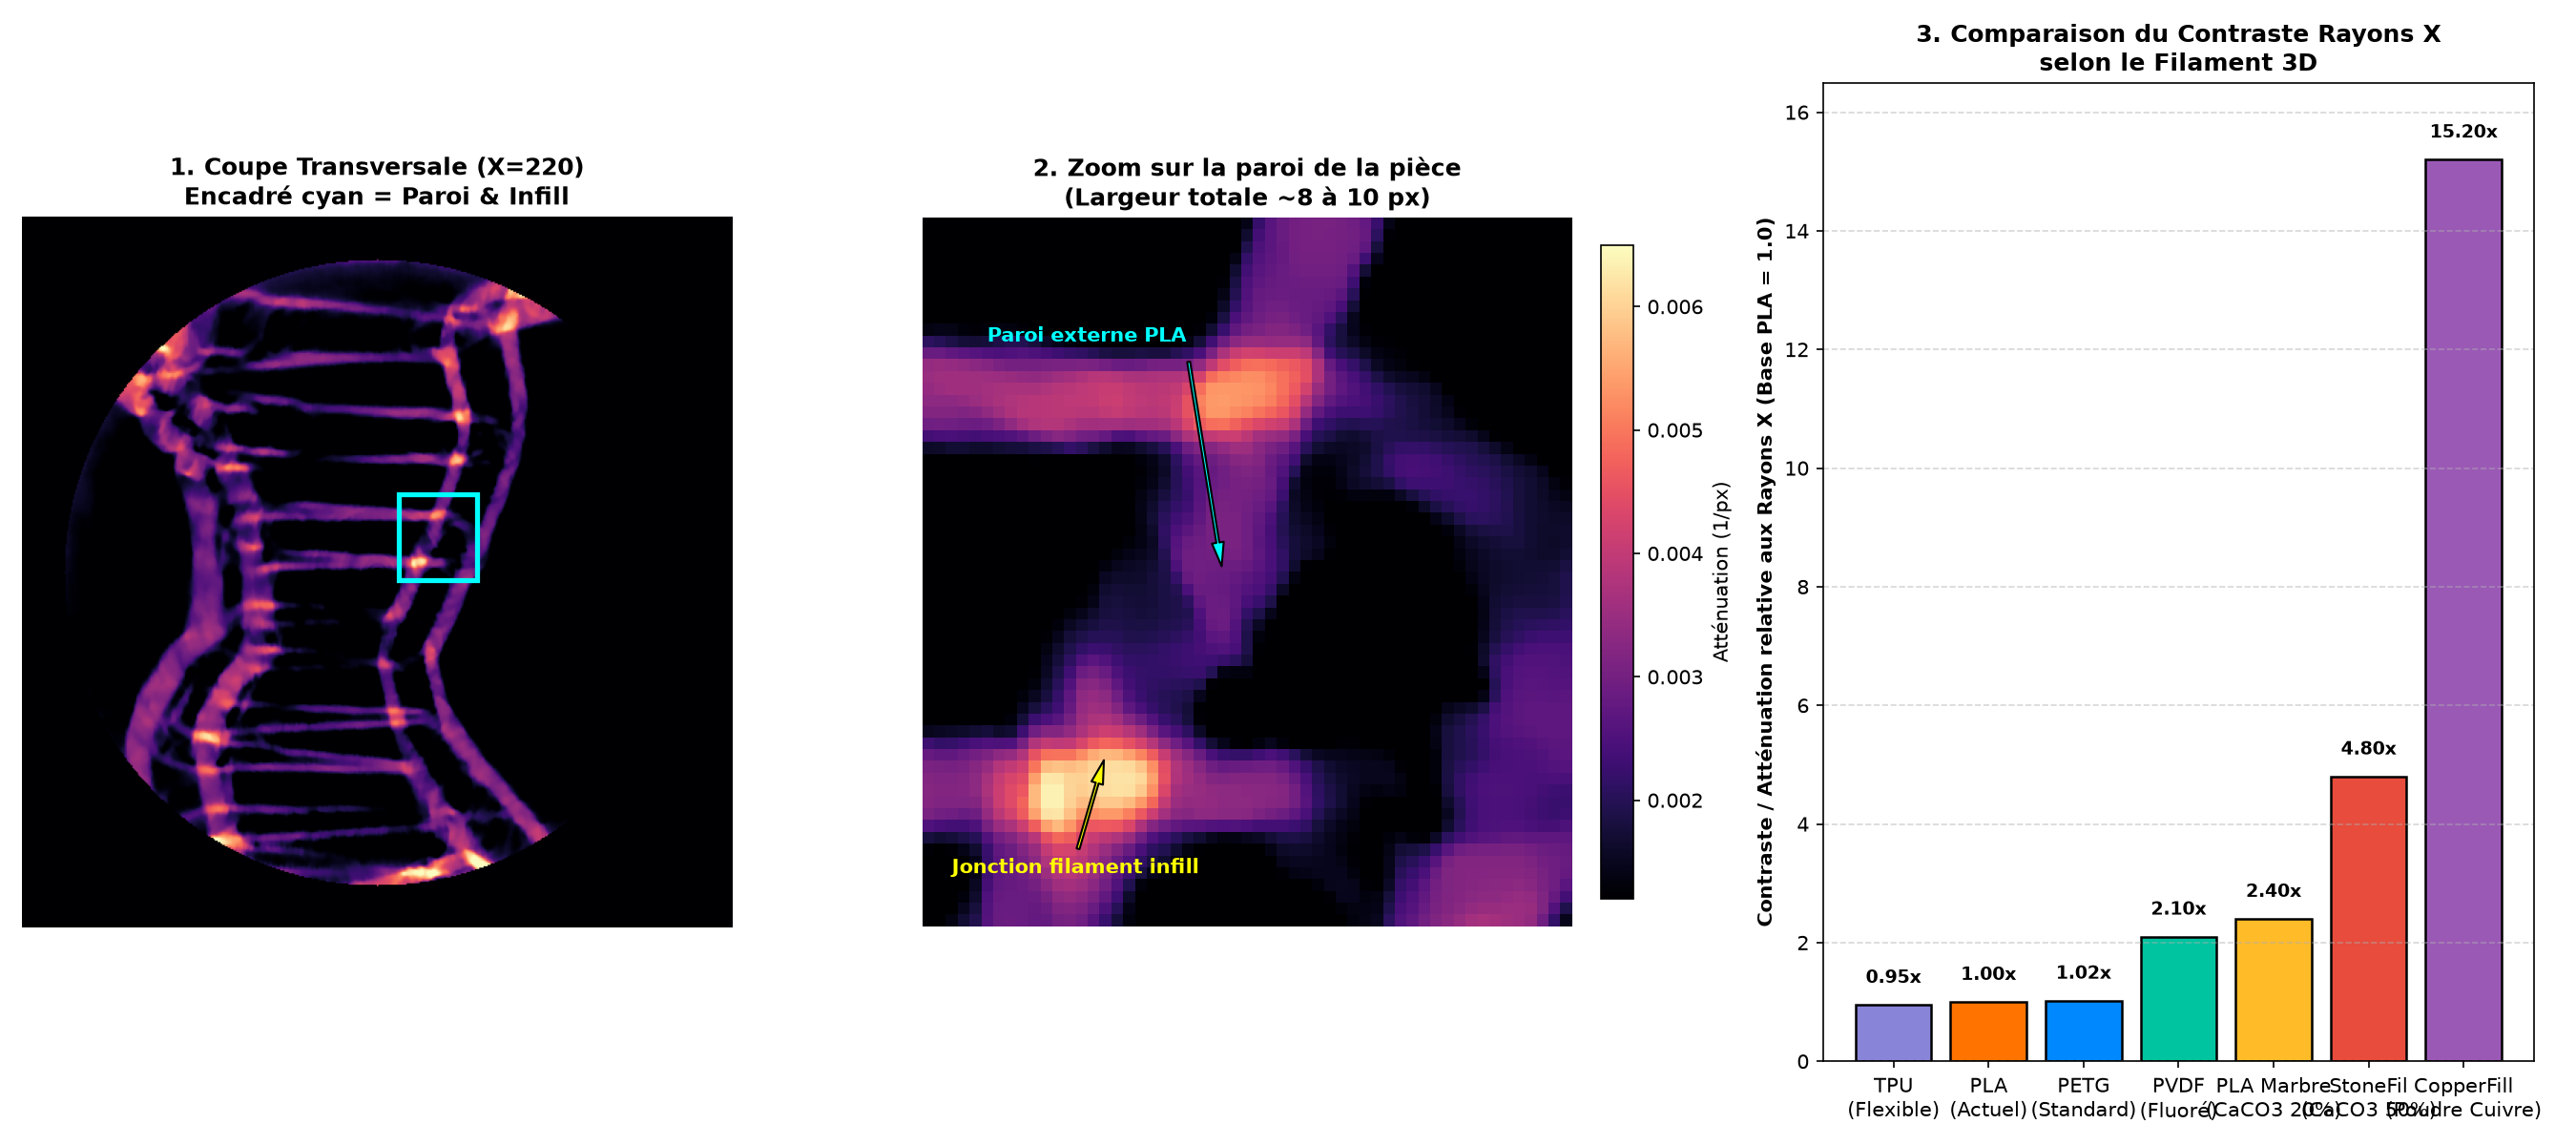
\includegraphics[width=0.70\linewidth]{figures/comparatif_materiaux_attenuation.png}
\caption{Étude comparative du contraste radiologique des polymères à basse énergie ($20 \text{ à } 35~\text{keV}$). À gauche et au centre~: visualisation de la coquille dense et des ancrages. À droite~: coefficient d'atténuation photoélectrique relatif normalisé par rapport au PLA standard ($1{,}00\times$). Le PETG ($1{,}02\times$), le TPU ($0{,}95\times$) et le PETG-CF ($0{,}87\times$) présentent un contraste similaire ou inférieur, tandis que les filaments chargés en carbonate de calcium (StoneFil, $2{,}4\times \text{ à } 4{,}8\times$) ou en particules métalliques (CopperFill, $12{,}5\times$) décuplent le contraste radiologique.}
\label{fig:comparatif_materiaux_attenuation}
\end{figure}

Les calculs théoriques fondés sur l'équation de Bragg-Pierce~\eqref{eq:bragg_pierce} démontrent que le PETG standard n'accroît le contraste que de $+2\,\%$, tandis que le TPU et le PETG chargé en fibres de carbone (PETG-CF) réduisent respectivement le contraste de $-5\,\%$ et $-13\,\%$ par rapport au PLA, en raison de la diminution de la fraction massique d'oxygène ($Z = 8$) au profit du carbone ($Z = 6$). 

En revanche, les filaments chargés en carbonate de calcium ($\text{CaCO}_3$, $Z_{\text{Ca}} = 20$) tels que le PLA Marbre et le StoneFil multiplient le contraste par un facteur de $2{,}4 \text{ à } 4{,}8$, constituant le choix optimal pour maximiser le contraste des détails sub-millimétriques lors des prochains étalonnages.
